\documentclass{article}
\usepackage[utf8]{inputenc}
\usepackage{siunitx}
\usepackage{graphics}
\usepackage[american,siunitx]{circuitikz}
\usepackage{amsmath}
\usepackage{svg} 
\usepackage{booktabs}
\usepackage{float}
\usepackage{xparse, xfp}
\usepackage{graphicx} 
\usepackage{steinmetz}
\usepackage{multirow}
\usepackage{pdfpages}
\usepackage{adjustbox}
%\renewcommand{\thesubsection}{\thesection.\alph{subsection}}
\newcommand{\equal}{=}
\newcommand*\circled[1]{\tikz[baseline=(char.base)]{
    \node[shape=circle,draw,inner sep=1pt] (char) {#1};}}

\title{ECE2101L\\Electrical Circuit Analysis II Laboratory\\\,\\Lab 10\\Resonance Circuits\\\,\\Report\\}
\author{Choi Tim Antony Yung}
%\author{Choi Tim Antony Yung\\\,\\Willis Nguyen\\Phineas Cozmiuc}

\begin{document}

\clearpage\maketitle
\thispagestyle{empty}
\newpage
\setcounter{page}{1}


\section{Series resonance}
\begin{center}
    \begin{adjustbox}{max width=\textwidth}
        \begin{circuitikz}
            \draw
            (0,0) to[voltage source, v_=$v$] (0,-4)
            (0,0) to[short,i=$i$] ++(1,0) node[ocirc]{} node[above]{1}
                to[R=$R$] ++(3,0)
                to[L=$L$] ++(1.25,0) -- ++(1,0)
                to[C=$C$] ++(0,-4) -- (0,-4)
            (1,-4) node[ocirc]{}
            (3.5,0) node[ocirc]{} node[above]{2}
            (5.75,0) node[ocirc]{} node[above]{3}
            (6.25,-3) node[ocirc]{} node[right]{4}
            ;
        \end{circuitikz}
    \end{adjustbox}
\end{center}

\subsection*{Procedure}
The above circuit was simulated with MATLAB R2019a with the RMS value of source voltage.

\subsection*{Result}
\begin{table}[H]
    \resizebox{\columnwidth}{!}{%
    \begin{tabular}{rrcccccc}
        \toprule
        &Frequency & $|i(t)|$ RMS & $|i(t)|$ RMS & $|V_{12}|$ RMS & $|V_{12}|$ RMS & $|V_{23}|$ RMS & $|V_{34}|$ RMS \\
        && calculated & measured & calculated & measured & measured & measured \\
        \midrule
        $f_0-110=$&\SI{54.15579}{\hertz} &\SI{6.126741}{\milli\ampere}&\SI{6.127}{\milli\ampere}&\SI{0.9190111}{\volt}&\SI{0.9190}{\volt}&\SI{0.4170}{\volt}&\SI{3.831}{\volt}\\
        $f_0-80=$ &\SI{84.15579}{\hertz} &\SI{10.63645}{\milli\ampere}&\SI{10.64}{\milli\ampere}&\SI{1.595467 }{\volt}&\SI{1.595 }{\volt}&\SI{1.125 }{\volt}&\SI{4.280}{\volt}\\
        $f_0-50=$ &\SI{114.15579}{\hertz}&\SI{16.49073}{\milli\ampere}&\SI{16.49}{\milli\ampere}&\SI{2.473610 }{\volt}&\SI{2.474 }{\volt}&\SI{2.366 }{\volt}&\SI{4.892}{\volt}\\
        $f_0=$    &\SI{164.15579}{\hertz}&\SI{23.57023}{\milli\ampere}&\SI{23.57}{\milli\ampere}&\SI{3.535534 }{\volt}&\SI{3.536 }{\volt}&\SI{4.862 }{\volt}&\SI{4.862}{\volt}\\
        $f_0+50=$ &\SI{214.15579}{\hertz}&\SI{18.94709}{\milli\ampere}&\SI{18.95}{\milli\ampere}&\SI{2.842064 }{\volt}&\SI{2.842 }{\volt}&\SI{5.099 }{\volt}&\SI{2.996}{\volt}\\
        $f_0+80=$ &\SI{244.15579}{\hertz}&\SI{15.69180}{\milli\ampere}&\SI{15.69}{\milli\ampere}&\SI{2.353770 }{\volt}&\SI{2.354 }{\volt}&\SI{4.814 }{\volt}&\SI{2.176}{\volt}\\
        $f_0+110=$&\SI{274.15579}{\hertz}&\SI{13.23696}{\milli\ampere}&\SI{13.24}{\milli\ampere}&\SI{1.985544 }{\volt}&\SI{1.986 }{\volt}&\SI{4.560 }{\volt}&\SI{1.635}{\volt}\\
        \bottomrule    
    \end{tabular} }
\end{table}


\subsection*{Analysis}
From the plot below it can be observed that the current and voltage of the resistor is at its maximum at the resonance frequency. This is due to that the magnitude of the impedance is at its maximum at resonance frequency when the impedance is purely real and thus all the power is dissipated through the resistor. At the resonance frequency, as the reactive impedance cancel each other out, with the voltage of inductor and capacitor being equal and opposite, the impedance of the RLC circuit is equal to that of the resistor, hence the voltage of the resistor is the same as the one of the voltage sourve.

\newpage
\begin{figure}[H]
    \centering
        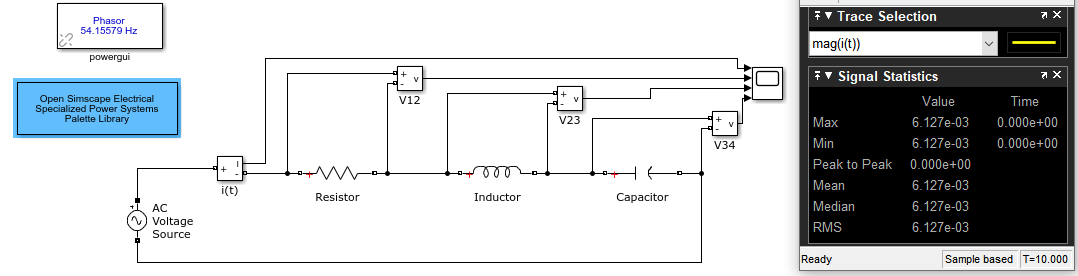
\includegraphics[width=\textwidth]{ECE2101L_Lab10_B1.png}
        \caption{Simulation of the circuit}
\end{figure}
\begin{figure}[H]
    \centering
        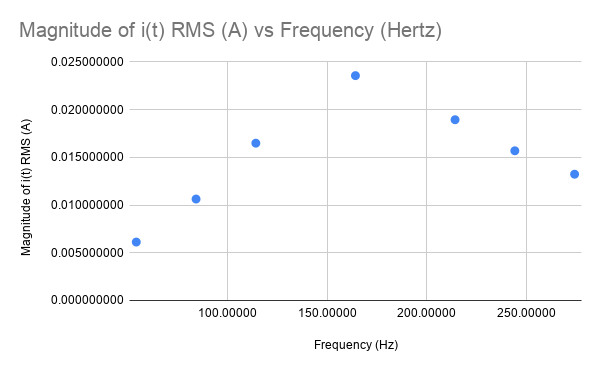
\includegraphics[scale=0.45]{ECE2101L_Lab10_B1_plot1.png}
        \caption{Measured RMS magnitude of i(t) versus frequency}
\end{figure}
\begin{figure}[H]
    \centering
        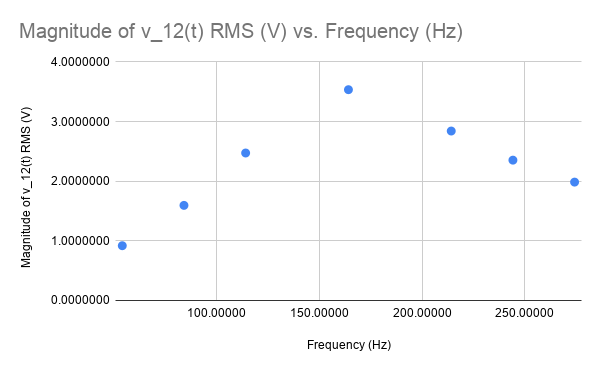
\includegraphics[scale=0.45]{ECE2101L_Lab10_B1_plot2.png}
        \caption{Measured $V_{12}$ RMS versus frequency}
\end{figure}

\newpage

\section{Parallel resonance}

\begin{center}
    \begin{circuitikz}
        \draw
        (0,0) to[voltage source, l_=$v$] (0,-3)
        (0,0) to[short, i=$i$] ++(1,0) node[ocirc]{} -- ++(1,0) node[circ](R){} -- ++(1.5,0) node[circ](L){} -- ++(1.5,0) to[C=$C$, i>_=$i_3$] ++(0,-3) -- (0,-3)
        (1,-3)node[ocirc]{}
        (R) to[R=$R$, i>_=$i_1$] ++(0,-3) node[circ]{}
        (L) to[L=$L$, i>_=$i_2$] ++(0,-3) node[circ]{}
        ;
    \end{circuitikz}
\end{center}

\subsection*{Procedure}
The above circuit was simulated with MATLAB R2019a with the RMS value of source voltage. A very small resistor was put in series to the circuit such that the simulation can go forward.

\subsection*{Result}
\begin{table}[H]
    \resizebox{\columnwidth}{!}{%
    \begin{tabular}{rrccccc}
        \toprule
        &Frequency & $|i_1(t)|$ RMS & $|i_2(t)|$ RMS & $|i_3(t)|$ RMS & $|i(t)|$ RMS & $|i(t)|$ RMS \\
        && calculated & calculated & calculated & calculated & measured \\
        \midrule
        $f=$    &\SI{60}{\hertz}&\SI{23.57023}{\milli\ampere}&\SI{46.89147}{\milli\ampere}&\SI{6.264465}{\milli\ampere}&\SI{46.96924}{\milli\ampere}&\SI{46.84}{\milli\ampere} \\
        $f_0=$    &\SI{164.15579}{\hertz}&\multicolumn{4}{c}{No calculation}&\SI{23.31}{\milli\ampere} \\
        \bottomrule
    \end{tabular} }
\end{table}

\subsection*{Analysis}
The total current is not the same in normal frequency than when the circuit is in resonance. In resonance, the impedance is purely resistive as the two reactive component cancel each other out. However, in normal frequency, there is a non-zero reactive impedance, therefore the magnitude of the impedance is smaller at normal frequency than at resonance frequency, which further implies that there is a larger current at normal frequency than at resonance frequency.

\newpage

\begin{figure}[H]
    \centering
        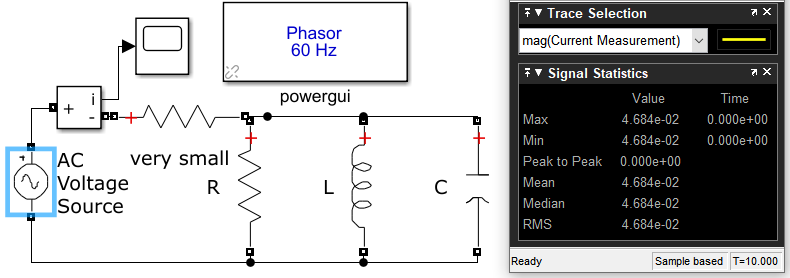
\includegraphics[width=\textwidth]{ECE2101L_Lab10_B2_60.png}
        \caption{Simulation of the circuit at \SI{60}{\hertz}}
\end{figure}

\begin{figure}[H]
    \centering
        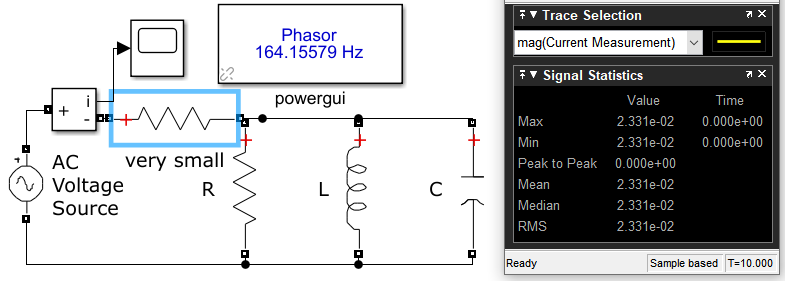
\includegraphics[width=\textwidth]{ECE2101L_Lab10_B2_f0.png}
        \caption{Simulation of the circuit in resonance}
\end{figure}

\end{document}

